% typ dokumentu beamer (knižnica) slúži na vytvorenie prezentácií
\documentclass{beamer}

% definovanie slovenskeho jazyka
% \usepackage[utf8x]{inputenc}
% \usepackage[slovak]{babel}

\usepackage[utf8]{inputenc}
\usepackage[T1]{fontenc}
\usepackage{lipsum, lmodern}

% definicia vzhladu prezentacie (zakladne temy najdete na: https://deic.uab.cat/~iblanes/beamer_gallery/index_by_theme.html)
%\usetheme{Singapore}
\usetheme{CambridgeUS}

% cesta k obrazkam, ktore su v prezentacii
\graphicspath{ {pics/} }

% informacie o prezentacii (nazov, autor, institut, datum)
\title{Ako písať v \LaTeX u}
\subtitle{prezentáciu}
\author{meno priezvisko}

\institute[STU] % volitelne
{
  vedúci práce \\
  odbor/pracovisko/škola
}

\date{\today}

% zobrazenie obsahu pred kazdym zaciatkom sekcie
 \AtBeginSection[]
 {
 \begin{frame}
    % \frametitle{\textbf{Obsah}}
    \tableofcontents[currentsection]
 \end{frame}
 }

% zaciatok prezentacie
\begin{document}

% vytvorenie uvodneho slidu
\begin{frame}
\titlepage
\end{frame}

% slide s obsahom 
% \begin{frame}
% 	\tableofcontents
% \end{frame}

% nazov casti prezentacie, ktora zacina
\section{úvod}

\begin{frame}{Nadpis}{podnadpis}
\begin{center}
Text na prvom slide.
\end{center}
\end{frame}

\section{zoznam}

\subsection{číslovaný}
\begin{frame}{zoznam}{číslovaný}
\begin{enumerate}
    \item prvá položka
    \item druhá položka
\end{enumerate}
\end{frame}

% nazov sub-casti prezentacie, ktora zacina
\subsection{nečíslovaný}

\begin{frame}{zoznam}{nečíslovaný}
\begin{itemize}
    \item prvá položka
    \item druhá položka
\end{itemize}
\end{frame}

\subsubsection{postupne pribúdajúci}

\begin{frame}{zoznam}{postupne pribúdajúci}
\begin{itemize}
    \item<1-1> prvá položka
    \item<2-> druhá položka
    \item<3-> tretia položka
\end{itemize}
\end{frame}

\section{rovnice}

\begin{frame}{rovnice}
\begin{itemize}
    \item výraz, ktorý je nie je definovaný ako matematický c = a+b
    \item výraz, ktorý je súčasťou riadku $c = a+b$
    \item výraz, uvedený na novom riadku $$c = a+b$$
    \item výraz, uvedený na novom riadku (iný spôsob) 
    \begin{equation*}
        c = a+b
    \end{equation*}
    \item výraz, uvedený na novom riadku (iný spôsob) - očíslovaný ku~ktorému~sa dá následne referovať
    \begin{equation}
        c = a+b
    \end{equation}
\end{itemize}
\end{frame}

\section{obrázoky}

\begin{frame}{obrázok}{jeden}
\begin{center}
    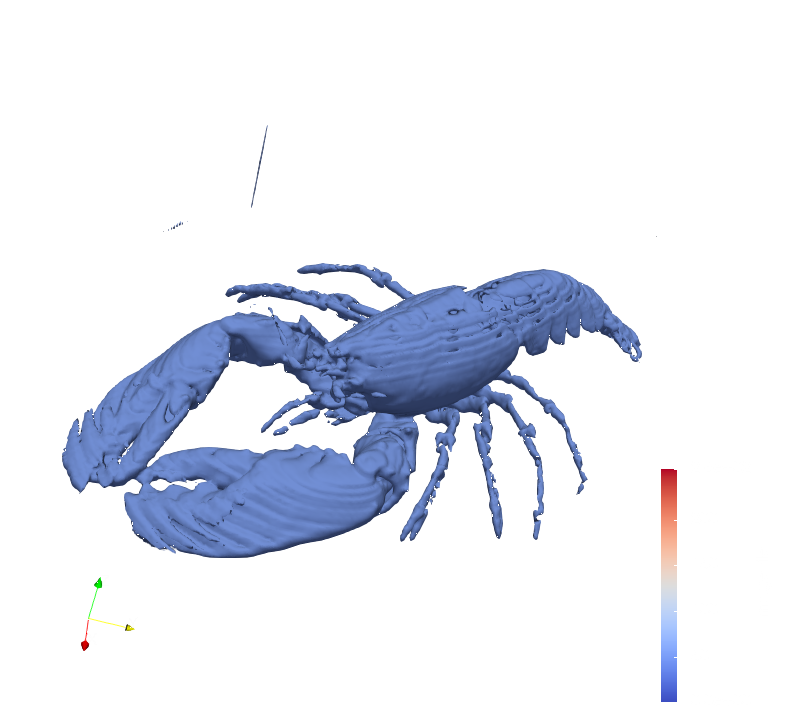
\includegraphics[width= .5 \linewidth]{lobster.png}    
\end{center}


\end{frame}

\begin{frame}{obrázky}{dva vedľa seba}

\begin{figure}
	\centering
      \subfloat{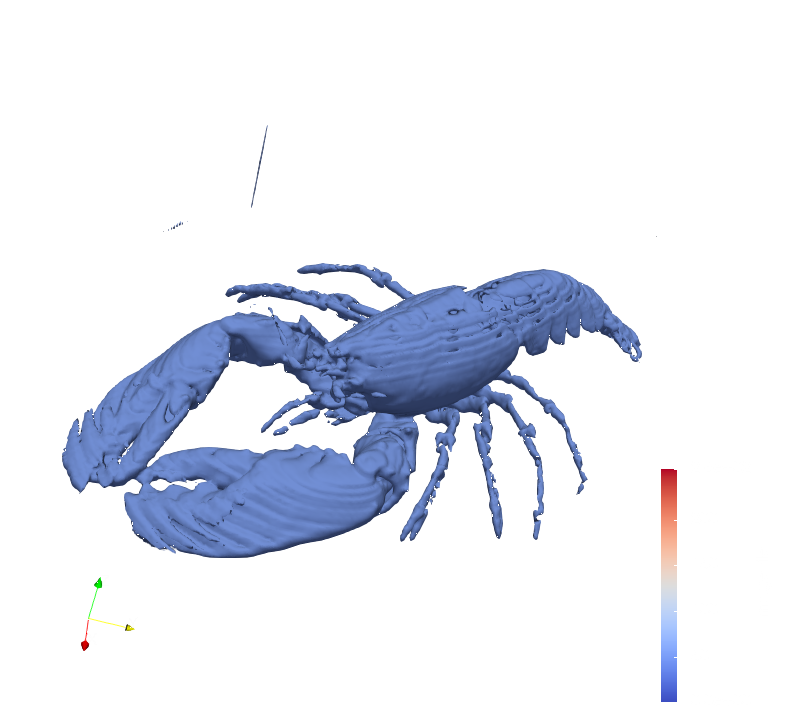
\includegraphics[width= 0.35 \linewidth]{lobster.png}}
      \qquad
    \subfloat{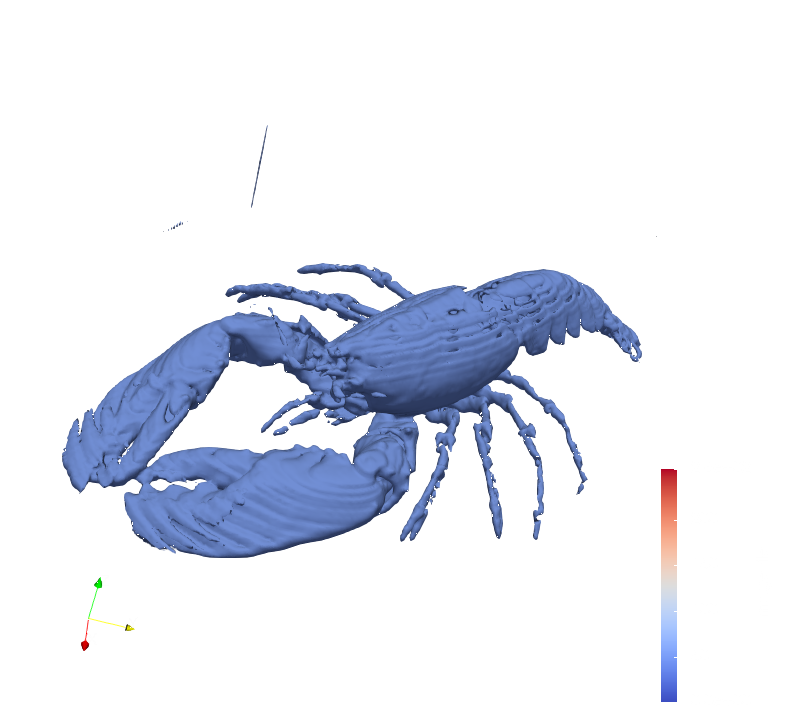
\includegraphics[width= 0.35 \linewidth]{lobster.png}}
\end{figure}

\end{frame}

\section{tabuľka}

\begin{frame}{tabuľka}

\begin{itemize} 
    \item neohraničená tabuľka \\
            \vspace{2em}
        \begin{tabular}{ l c r }
          1 & 2 & 3 \\
          4 & 5 & 6 \\
          7 & 8 & 9 \\
        \end{tabular}
        \vspace{2em}
    \item ohraničená tabuľka \\
            \vspace{2em}
                \begin{tabular}{| l | c | r | }
                \hline
          1 & 2 & 3 \\ \hline
          4 & 5 & 6 \\ \hline
          7 & 8 & 9 \\
          \hline
        \end{tabular}
\end{itemize}

\end{frame}


\frame{
Ďakujem za pozotnosť!}

\end{document}